\chapter{Continual Learning with Background Knowledge}
\label{chap:zincontinual}

Traditional settings in Continual Learning are framed within a knowledge agnostic scenario, where catastrophic forgetting must be counteracted in a generic fashion. However, many real world applications are characterized by known temporal dynamics (e.g., outdoor security cameras are subject to cyclic day-night domain shifts). In this chapter we exploit the \textsc{LTLZinc-Continual} datasets to adapt traditional, knowledge agnostic, Continual Learning strategies to a setting where background knowledge can be exploited for better concept retention. Our adaptation is based on segregating the ``memory'' (i.e., a replay buffer, or a subset of trainable parameters) available for each strategy into discrete \textit{knowledge units}, enabled according to available temporal knowledge.
%
The content of chapter is adapted from our journal paper under review at JAIR~\cite{lorello2025ltlzinc}.

\section{Methodology}
We address the Class-continual learning tasks of \textsc{LTLZinc-Continual} by means of Convolutional Neural Networks, augmented (only at training-time) by a combination of strategies, representing the main categories of replay-based, regularization-based and architecture-based Continual Learning. Appendix~\ref{app:ltlzinccont} provides additional information to reproduce our experiments.
%
\paragraph{Architecture.} The architecture is composed of a GoogLeNet~\cite{szegedy2015going} backbone, equipped with a classification head, comprised of: a linear embedding layer of $emb\_size$ neurons, a dictionary of hidden blocks (linear layer of $hidden\_size$ neurons, followed by ReLU activations), and a linear classification neuron for each class.
If the architecture-based strategy is not active, the dictionary contains a single hidden block, acting as simple reprojection of the embedding layer, otherwise, it is composed of an independent hidden block for each of the injected \textit{knowledge units}, and the output tensors are concatenated before being passed to the classification layer.
In the \textsc{LTLZinc-Continual-MNIST} variant, the backbone is initialized with random weights, while for \textsc{LTLZinc-Continual-CIFAR}, the backbone is initialized with weights pre-trained on ImageNet~\cite{russakovsky2015imagenet}. For \textsc{CIFAR-100} experiments we also explore the effect of freezing the backbone (training only the downstream linear embedding, hidden blocks and linear classifier layers).

\paragraph{Continual Learning Strategies.} We address the catastrophic forgetting problem with multiple combinations of Continual Learning strategies, enabled for different experiments. For the experience-replay family of strategies, we experiment with Class-balanced Reservoir Sampling~\cite{chrysakis2020online} associated with either a Categorical Cross-entropy loss, or a Gradient Episodic Memory (GEM)~\cite{lopez2017gradient} loss. In both cases, a replay buffer of fixed size is capable of storing up to $\text{buffer\_size} = 500$ previously observed image samples and their class labels, which can be read in batches of size $\text{buffer\_batch} = 16$. As a representative of regularization-based strategies, we implement Learning without Forgetting (LwF)~\cite{li2017learning}, as a form of self-distillation of the model prediction against both new and buffered data.

\paragraph{Knowledge-Injection.} We inject knowledge at the Continual Learning strategy level, by means of segregation with respect to $k$ \textbf{knowledge units}. In our experiments we focus on three families of units: \textbf{None} (traditional Continual Learning baseline), \textbf{Predicates} and \textbf{States}.
Predicate-level units are a form of ``high-level'' knowledge, defining a partition based on which constraints in $\gC$ are true in the current episode, while state-level units partition based on the automaton state corresponding to the current episode (and are thus at a lower level of abstraction, compared to predicate units).
%
Knowledge is injected in replay-based strategies by reserving $\lfloor \frac{\text{buffer\_size}}{k}\rfloor$ samples for each knowledge unit. The Gradient Episodic Memory algorithm is modified to take into account knowledge units, instead of class labels during its quadratic programming step. 
Learning without Forgetting is modified into a form of teacher-student distillation, by keeping in memory $k$ copies of the neural architecture, each of which is trained only on image samples corresponding to their own knowledge unit.
The modular architecture-based strategy natively supports knowledge injection, as each of the hidden blocks already corresponds to a different knowledge unit.
%
It is important to note that in our setting it is not possible to inject knowledge onto the Naive combination, where no strategy is active, as knowledge units interact only with Continual Learning strategies.

\paragraph{Training.} At the beginning of each episode, an oracular controller determines the subset of knowledge units active for the episode,\footnote{For the \textbf{None} injection level, a single dummy knowledge unit is always kept active.} based on auxiliary \textsc{LTLZinc} annotations (i.e., current automaton state and constraint truth values).\footnote{In principle, the controller can be learned, instead of relying on ground truth annotations, e.g., following approaches for Continual Learning with unknown task boundaries~\cite{zhu2024continual}.} This subset will guide Continual Learning strategies during training.
The training loop for a single episode is composed of a (i.) \textit{setup phase}, a (ii.) \textit{training phase} and an (iii.) \textit{evaluation phase}.
In the \textit{setup phase}, the weights of hidden blocks corresponding to inactive knowledge units are frozen, and, if Learning without Forgetting is active with no background knowledge available (\textbf{None} setting), weights of the entire neural network are copied onto a single teacher for self-distillation during the training phase.
%
The general idea of the \textit{training phase} is to allow plasticity by updating \textbf{active knowledge units} with new samples, while regularizing the agent (which always learns from new samples) against \textbf{inactive knowledge units} to guarantee stability. To achieve this, a mini-batch is sampled from the current episode, processed by the replay-based and regularization-based strategies enabled for the current experiment, and finally used to train the Neural Network (along with additional objectives provided by Continual Learning strategies).
The replay buffers corresponding to currently active knowledge units stochastically store each observed image in the mini-batch, according to the Reservoir Sampling algorithm. Teachers corresponding to active knowledge units are trained against the mini-batch by means of Categorical cross-entropy.
The Convolutional Neural Network is trained on the mini-batch (Categorical Cross-entropy loss), as well as the following auxiliary objectives, when the corresponding strategy is enabled for the current experiment: Experience-replay loss on a buffered mini-batch, sampled from inactive knowledge units (Categorical cross-entropy, or GEM loss), Learning without Forgetting loss against inactive teachers (Kullback-Leibler Divergence, both on current and buffered mini-batches). Gradient is back-propagated to the backbone only through the hidden blocks corresponding to active knowledge units.
%
Finally, at the \textit{evaluation phase}, well-established metrics~\cite{mai2022online} in the Continual Learning literature are evaluated against training, validation and test sets.
\textsc{Average accuracy} is the average of the class-related accuracies at the end of learning, \textsc{Forward Transfer} measures the positive effect of learned features on yet-to-be-observed future episodes, and \textsc{Average Forgetting} is the difference between the current average accuracy (averaged over every past episode) and the best observed average accuracy in the past.
For Average Accuracy and Forgetting, we also focus their evaluation on the target classes specified for each task (i.e., rare classes for Task 1 and recurrent classes for Task 2). In the case in which an episode contains no such classes, focused episode-level accuracy is not defined, and discarded when computing global average accuracy and forgetting.
We perform model selection by measuring Average Accuracy at the end of training on the validation set.

\section{Results}
%\TODO{AAAA}
\begin{table}
	\centering
	\resizebox{\textwidth}{!}{
		\begin{tabular}{ccccccccccc}
			\toprule
			\multirow{3}{*}{\sc Task} & \multirow{3}{*}{\shortstack[c]{\sc Knowledge\\\sc Availability}} & \multirow{3}{*}{\sc Category} & \multirow{3}{*}{\sc Buffer} & \multirow{3}{*}{\sc Distillation} & \multirow{3}{*}{\sc Architecture} & \multirow{3}{*}{\shortstack[c]{\sc Average\\\sc Accuracy}\raisebox{1.5ex}{\:$\uparrow$}} & \multirow{3}{*}{\shortstack[c]{\sc Average\\\sc Forgetting}\raisebox{1.5ex}{\:$\downarrow$}} & \multirow{3}{*}{\shortstack[c]{\sc Forward\\\sc Transfer}\raisebox{1.5ex}{\:$\uparrow$}} & \multirow{3}{*}{\shortstack[c]{\sc Focused\\\sc Average\\\sc Accuracy}\raisebox{2.5ex}{\:$\uparrow$}} & \multirow{3}{*}{\shortstack[c]{\sc Focused\\\sc Average\\\sc Forgetting}\raisebox{2.5ex}{\:$\downarrow$}} \\
			& & & & & & & & & & \\
			& & & & & & & & & & \\
			\midrule
			%Task 1 (MNIST) & Predicates & Naive & No buffer & No distillation & Flat & $0.88 $ {\tiny ($\pm 0.01$)} & $0.11 $ {\tiny ($\pm 0.00$)} & $0.53 $ {\tiny ($\pm 0.02$)} & $0.00 $ {\tiny ($\pm 0.00$)} & $1.00 $ {\tiny ($\pm 0.00$)}\\
			\multirow{14}{*}{\shortstack[c]{Task 1\\(MNIST)}} & \multirow{5}{*}{Predicates} & Replay & Reservoir (CCE) & No distillation & Flat & $0.95 $ {\tiny ($\pm 0.02$)} & $\textbf{0.03} $ {\tiny ($\pm 0.02$)} & $\textbf{0.70} $ {\tiny ($\pm 0.03$)} & $0.71 $ {\tiny ($\pm 0.22$)} & $0.26 $ {\tiny ($\pm 0.22$)}\\
			&  & Modular & No buffer & No distillation & Modular & $0.88 $ {\tiny ($\pm 0.01$)} & $0.11 $ {\tiny ($\pm 0.00$)} & $0.51 $ {\tiny ($\pm 0.02$)} & $0.00 $ {\tiny ($\pm 0.00$)} & $1.00 $ {\tiny ($\pm 0.00$)}\\
			&  & Replay + Distillation & Reservoir (CCE) & Teacher-distillation & Flat & $0.95 $ {\tiny ($\pm 0.02$)} & $\textbf{0.03} $ {\tiny ($\pm 0.02$)} & $0.68 $ {\tiny ($\pm 0.04$)} & $\textbf{0.78} $ {\tiny ($\pm 0.23$)} & $\textbf{0.20} $ {\tiny ($\pm 0.22$)}\\
			&  & Replay + Modular & Reservoir (CCE) & No distillation & Modular & $\textbf{0.96} $ {\tiny ($\pm 0.02$)} & $\textbf{0.03} $ {\tiny ($\pm 0.03$)} & $\textbf{0.70} $ {\tiny ($\pm 0.03$)} & $0.77 $ {\tiny ($\pm 0.23$)} & $0.21 $ {\tiny ($\pm 0.25$)}\\
			&  & All & Reservoir (CCE) & Teacher-distillation & Modular & $0.95 $ {\tiny ($\pm 0.03$)} & $\textbf{0.03} $ {\tiny ($\pm 0.03$)} & $0.67 $ {\tiny ($\pm 0.03$)} & $0.76 $ {\tiny ($\pm 0.26$)} & $0.24 $ {\tiny ($\pm 0.26$)}\\
			\cdashline{2-11}
			%Task 1 (MNIST) & States & Naive & No buffer & No distillation & Flat & $0.88 $ {\tiny ($\pm 0.00$)} & $0.12 $ {\tiny ($\pm 0.00$)} & $0.54 $ {\tiny ($\pm 0.01$)} & $0.00 $ {\tiny ($\pm 0.00$)} & $1.00 $ {\tiny ($\pm 0.00$)}\\
			& \multirow{5}{*}{States} & Replay & Reservoir (CCE) & No distillation & Flat & $\textbf{0.97} $ {\tiny ($\pm 0.00$)} & $\textbf{0.01} $ {\tiny ($\pm 0.01$)} & $\textbf{0.66} $ {\tiny ($\pm 0.02$)} & $\textbf{0.89} $ {\tiny ($\pm 0.05$)} & $\textbf{0.09} $ {\tiny ($\pm 0.06$)}\\
			&  & Modular & No buffer & No distillation & Modular & $0.88 $ {\tiny ($\pm 0.00$)} & $0.11 $ {\tiny ($\pm 0.01$)} & $0.52 $ {\tiny ($\pm 0.01$)} & $0.00 $ {\tiny ($\pm 0.00$)} & $1.00 $ {\tiny ($\pm 0.00$)}\\
			&  & Replay + Distillation & Reservoir (GEM) & Teacher-distillation & Flat & $0.95 $ {\tiny ($\pm 0.01$)} & $0.03 $ {\tiny ($\pm 0.01$)} & $0.58 $ {\tiny ($\pm 0.02$)} & $0.79 $ {\tiny ($\pm 0.06$)} & $0.21 $ {\tiny ($\pm 0.06$)}\\
			&  & Replay + Modular & Reservoir (GEM) & No distillation & Modular & $0.96 $ {\tiny ($\pm 0.01$)} & $0.03 $ {\tiny ($\pm 0.02$)} & $0.58 $ {\tiny ($\pm 0.03$)} & $0.76 $ {\tiny ($\pm 0.08$)} & $0.24 $ {\tiny ($\pm 0.08$)}\\
			&  & All & Reservoir (CCE) & Teacher-distillation & Modular & $0.96 $ {\tiny ($\pm 0.01$)} & $0.02 $ {\tiny ($\pm 0.01$)} & $0.65 $ {\tiny ($\pm 0.02$)} & $0.87 $ {\tiny ($\pm 0.05$)} & $0.12 $ {\tiny ($\pm 0.05$)}\\
			\cdashline{2-11}
			& \multirow{3}{*}{None} & Naive & No buffer & No distillation & Modular & $\textbf{0.88} $ {\tiny ($\pm 0.01$)} & $\textbf{0.11} $ {\tiny ($\pm 0.00$)} & $0.47 $ {\tiny ($\pm 0.03$)} & $0.00 $ {\tiny ($\pm 0.00$)} & $1.00 $ {\tiny ($\pm 0.00$)}\\
			&  & Replay & Reservoir (CCE) & No distillation & Flat & $\textbf{0.88} $ {\tiny ($\pm 0.01$)} & $\textbf{0.11} $ {\tiny ($\pm 0.01$)} & $0.50 $ {\tiny ($\pm 0.02$)} & $0.00 $ {\tiny ($\pm 0.00$)} & $1.00 $ {\tiny ($\pm 0.00$)}\\
			&  & Replay + Distillation & Reservoir (CCE) & Self-distillation & Flat & $\textbf{0.88} $ {\tiny ($\pm 0.00$)} & $0.12 $ {\tiny ($\pm 0.00$)} & $\textbf{0.53} $ {\tiny ($\pm 0.01$)} & $0.00 $ {\tiny ($\pm 0.00$)} & $1.00 $ {\tiny ($\pm 0.00$)}\\
			\midrule
			%Task 2 (MNIST) & Predicates & Naive & No buffer & No distillation & Flat & $0.51 $ {\tiny ($\pm 0.10$)} & $0.51 $ {\tiny ($\pm 0.11$)} & $0.31 $ {\tiny ($\pm 0.02$)} & $0.49 $ {\tiny ($\pm 0.21$)} & $0.53 $ {\tiny ($\pm 0.20$)}\\
			\multirow{14}{*}{\shortstack[c]{Task 2\\(MNIST)}} & \multirow{5}{*}{Predicates} & Replay & Reservoir (CCE) & No distillation & Flat & $\textbf{0.96} $ {\tiny ($\pm 0.01$)} & $\textbf{0.03} $ {\tiny ($\pm 0.01$)} & $\textbf{0.74} $ {\tiny ($\pm 0.02$)} & $\textbf{0.94} $ {\tiny ($\pm 0.02$)} & $\textbf{0.04} $ {\tiny ($\pm 0.03$)}\\
			&  & Modular & No buffer & No distillation & Modular & $0.49 $ {\tiny ($\pm 0.11$)} & $0.53 $ {\tiny ($\pm 0.12$)} & $0.31 $ {\tiny ($\pm 0.02$)} & $0.49 $ {\tiny ($\pm 0.24$)} & $0.53 $ {\tiny ($\pm 0.22$)}\\
			&  & Replay + Distillation & Reservoir (CCE) & Teacher-distillation & Flat & $0.92 $ {\tiny ($\pm 0.05$)} & $0.06 $ {\tiny ($\pm 0.05$)} & $0.66 $ {\tiny ($\pm 0.05$)} & $0.88 $ {\tiny ($\pm 0.09$)} & $0.10 $ {\tiny ($\pm 0.09$)}\\
			&  & Replay + Modular & Reservoir (CCE) & No distillation & Modular & $0.94 $ {\tiny ($\pm 0.05$)} & $0.05 $ {\tiny ($\pm 0.05$)} & $0.71 $ {\tiny ($\pm 0.03$)} & $0.91 $ {\tiny ($\pm 0.08$)} & $0.08 $ {\tiny ($\pm 0.08$)}\\
			&  & All & Reservoir (CCE) & Teacher-distillation & Modular & $0.92 $ {\tiny ($\pm 0.10$)} & $0.06 $ {\tiny ($\pm 0.09$)} & $0.63 $ {\tiny ($\pm 0.08$)} & $0.88 $ {\tiny ($\pm 0.16$)} & $0.09 $ {\tiny ($\pm 0.15$)}\\
			\cdashline{2-11}
			%Task 2 (MNIST) & States & Naive & No buffer & No distillation & Flat & $0.49 $ {\tiny ($\pm 0.12$)} & $0.53 $ {\tiny ($\pm 0.12$)} & $0.30 $ {\tiny ($\pm 0.03$)} & $0.48 $ {\tiny ($\pm 0.23$)} & $0.53 $ {\tiny ($\pm 0.21$)}\\
			& \multirow{5}{*}{States} & Replay & Reservoir (CCE) & No distillation & Flat & $\textbf{0.98} $ {\tiny ($\pm 0.00$)} & $\textbf{0.01} $ {\tiny ($\pm 0.00$)} & $\textbf{0.71} $ {\tiny ($\pm 0.03$)} & $\textbf{0.98} $ {\tiny ($\pm 0.01$)} & $0.02 $ {\tiny ($\pm 0.01$)}\\
			&  & Modular & No buffer & No distillation & Modular & $0.47 $ {\tiny ($\pm 0.12$)} & $0.55 $ {\tiny ($\pm 0.13$)} & $0.30 $ {\tiny ($\pm 0.02$)} & $0.47 $ {\tiny ($\pm 0.24$)} & $0.55 $ {\tiny ($\pm 0.22$)}\\
			&  & Replay + Distillation & Reservoir (CCE) & Teacher-distillation & Flat & $0.95 $ {\tiny ($\pm 0.02$)} & $0.03 $ {\tiny ($\pm 0.02$)} & $0.57 $ {\tiny ($\pm 0.11$)} & $0.94 $ {\tiny ($\pm 0.04$)} & $0.05 $ {\tiny ($\pm 0.04$)}\\
			&  & Replay + Modular & Reservoir (CCE) & No distillation & Modular & $\textbf{0.98} $ {\tiny ($\pm 0.01$)} & $\textbf{0.01} $ {\tiny ($\pm 0.00$)} & $0.70 $ {\tiny ($\pm 0.02$)} & $\textbf{0.98} $ {\tiny ($\pm 0.01$)} & $\textbf{0.01} $ {\tiny ($\pm 0.01$)}\\
			&  & All & Reservoir (CCE) & Teacher-distillation & Modular & $0.96 $ {\tiny ($\pm 0.02$)} & $0.02 $ {\tiny ($\pm 0.01$)} & $0.61 $ {\tiny ($\pm 0.07$)} & $0.95 $ {\tiny ($\pm 0.03$)} & $0.03 $ {\tiny ($\pm 0.03$)}\\
			\cdashline{2-11}
			& \multirow{3}{*}{None} & Naive & No buffer & No distillation & Flat & $\textbf{0.48} $ {\tiny ($\pm 0.11$)} & $\textbf{0.54} $ {\tiny ($\pm 0.12$)} & $\textbf{0.30} $ {\tiny ($\pm 0.02$)} & $\textbf{0.47} $ {\tiny ($\pm 0.25$)} & $\textbf{0.55} $ {\tiny ($\pm 0.23$)}\\
			& & Replay & Reservoir (GEM) & No distillation & Modular & $0.46 $ {\tiny ($\pm 0.11$)} & $0.56 $ {\tiny ($\pm 0.11$)} & $\textbf{0.30} $ {\tiny ($\pm 0.02$)} & $0.46 $ {\tiny ($\pm 0.25$)} & $0.56 $ {\tiny ($\pm 0.23$)}\\
			& & Replay + Distillation & Reservoir (CCE) & Self-distillation & Modular & $0.42 $ {\tiny ($\pm 0.09$)} & $0.60 $ {\tiny ($\pm 0.10$)} & $0.29 $ {\tiny ($\pm 0.01$)} & $0.42 $ {\tiny ($\pm 0.31$)} & $0.60 $ {\tiny ($\pm 0.29$)}\\
			\bottomrule
		\end{tabular}
	}
	\caption[Results on \textsc{LTLZinc-Continual-MNIST}]{Best \textsc{Average Accuracy}, \textsc{Average Forgetting} and \textsc{Forward Transfer} for Class-continual experiments on \textsc{LTLZinc-Continual-MNIST}, grouped by knowledge available to each strategy. Best models selected by \textsc{Average Accuracy} on validation set. Results are $mean \pm std$ over 9 runs (3 random seeds, times 3 different curricula).}
	\label{ltlzinc:tab:incremental-results-mnist}
\end{table}

\paragraph{\textsc{LTLZinc-Continual-MNIST}.} Table~\ref{ltlzinc:tab:incremental-results-mnist} highlights the best results on \textsc{LTLZinc-Continual-MNIST}. For both tasks, every method performs significantly above the random guessing threshold ($0.1$ accuracy), however methods employing knowledge injection (regardless of the level, predicates or states) have a clear advantage over baseline methods exploiting uninformed Continual Learning strategies. When used alone, the architecture-based strategy appears to interact negatively with knowledge injection: while in its uninformed version it performs on par (\textsc{Task 1}) or slightly better (\textsc{Task 2}) than other strategies, when combined with background knowledge, its performance drops significantly with respect to other strategies (by about $0.1$ for \textsc{Task 1} and $0.5$ for \textsc{Task 2}). This phenomenon can be explained by the fact that such strategy is characterized by additional training parameters, which receive gradients only when the corresponding hidden block is active, with the result that, compared to the uninformed baseline, for the same amount of data, each parameter receives only a fraction of the updates it would be subject to if trained naively.
With the exception of the modular architecture, every other strategy (or combination of strategies) performs equally well in terms of \textsc{Average Accuracy} and \textsc{Average Forgetting}, however, regularization-based methods (distillation alone, distillation and replay, or distillation and modular architecture), tend to be characterized by lower \textsc{Forward Transfer}.
Metrics focusing on target classes, highlight how not employing background knowledge (or relying only on architecture-based strategies) for \textsc{Task 1} has catastrophic outcomes: knowledge about the rare class is entirely erased by the end of training. For \textsc{Task 2}, on the other hand, where the classes of interest are those re-appearing periodically, the trend follows the same as global metrics. This behavior suggests the traditional evaluation protocols for fully-incremental settings, where all the classes are balanced across episodes and appear only once, can be potentially inadequate when adapted to more complex temporal behaviors.

\begin{figure}
	\centering
	\begin{minipage}{\linewidth}
		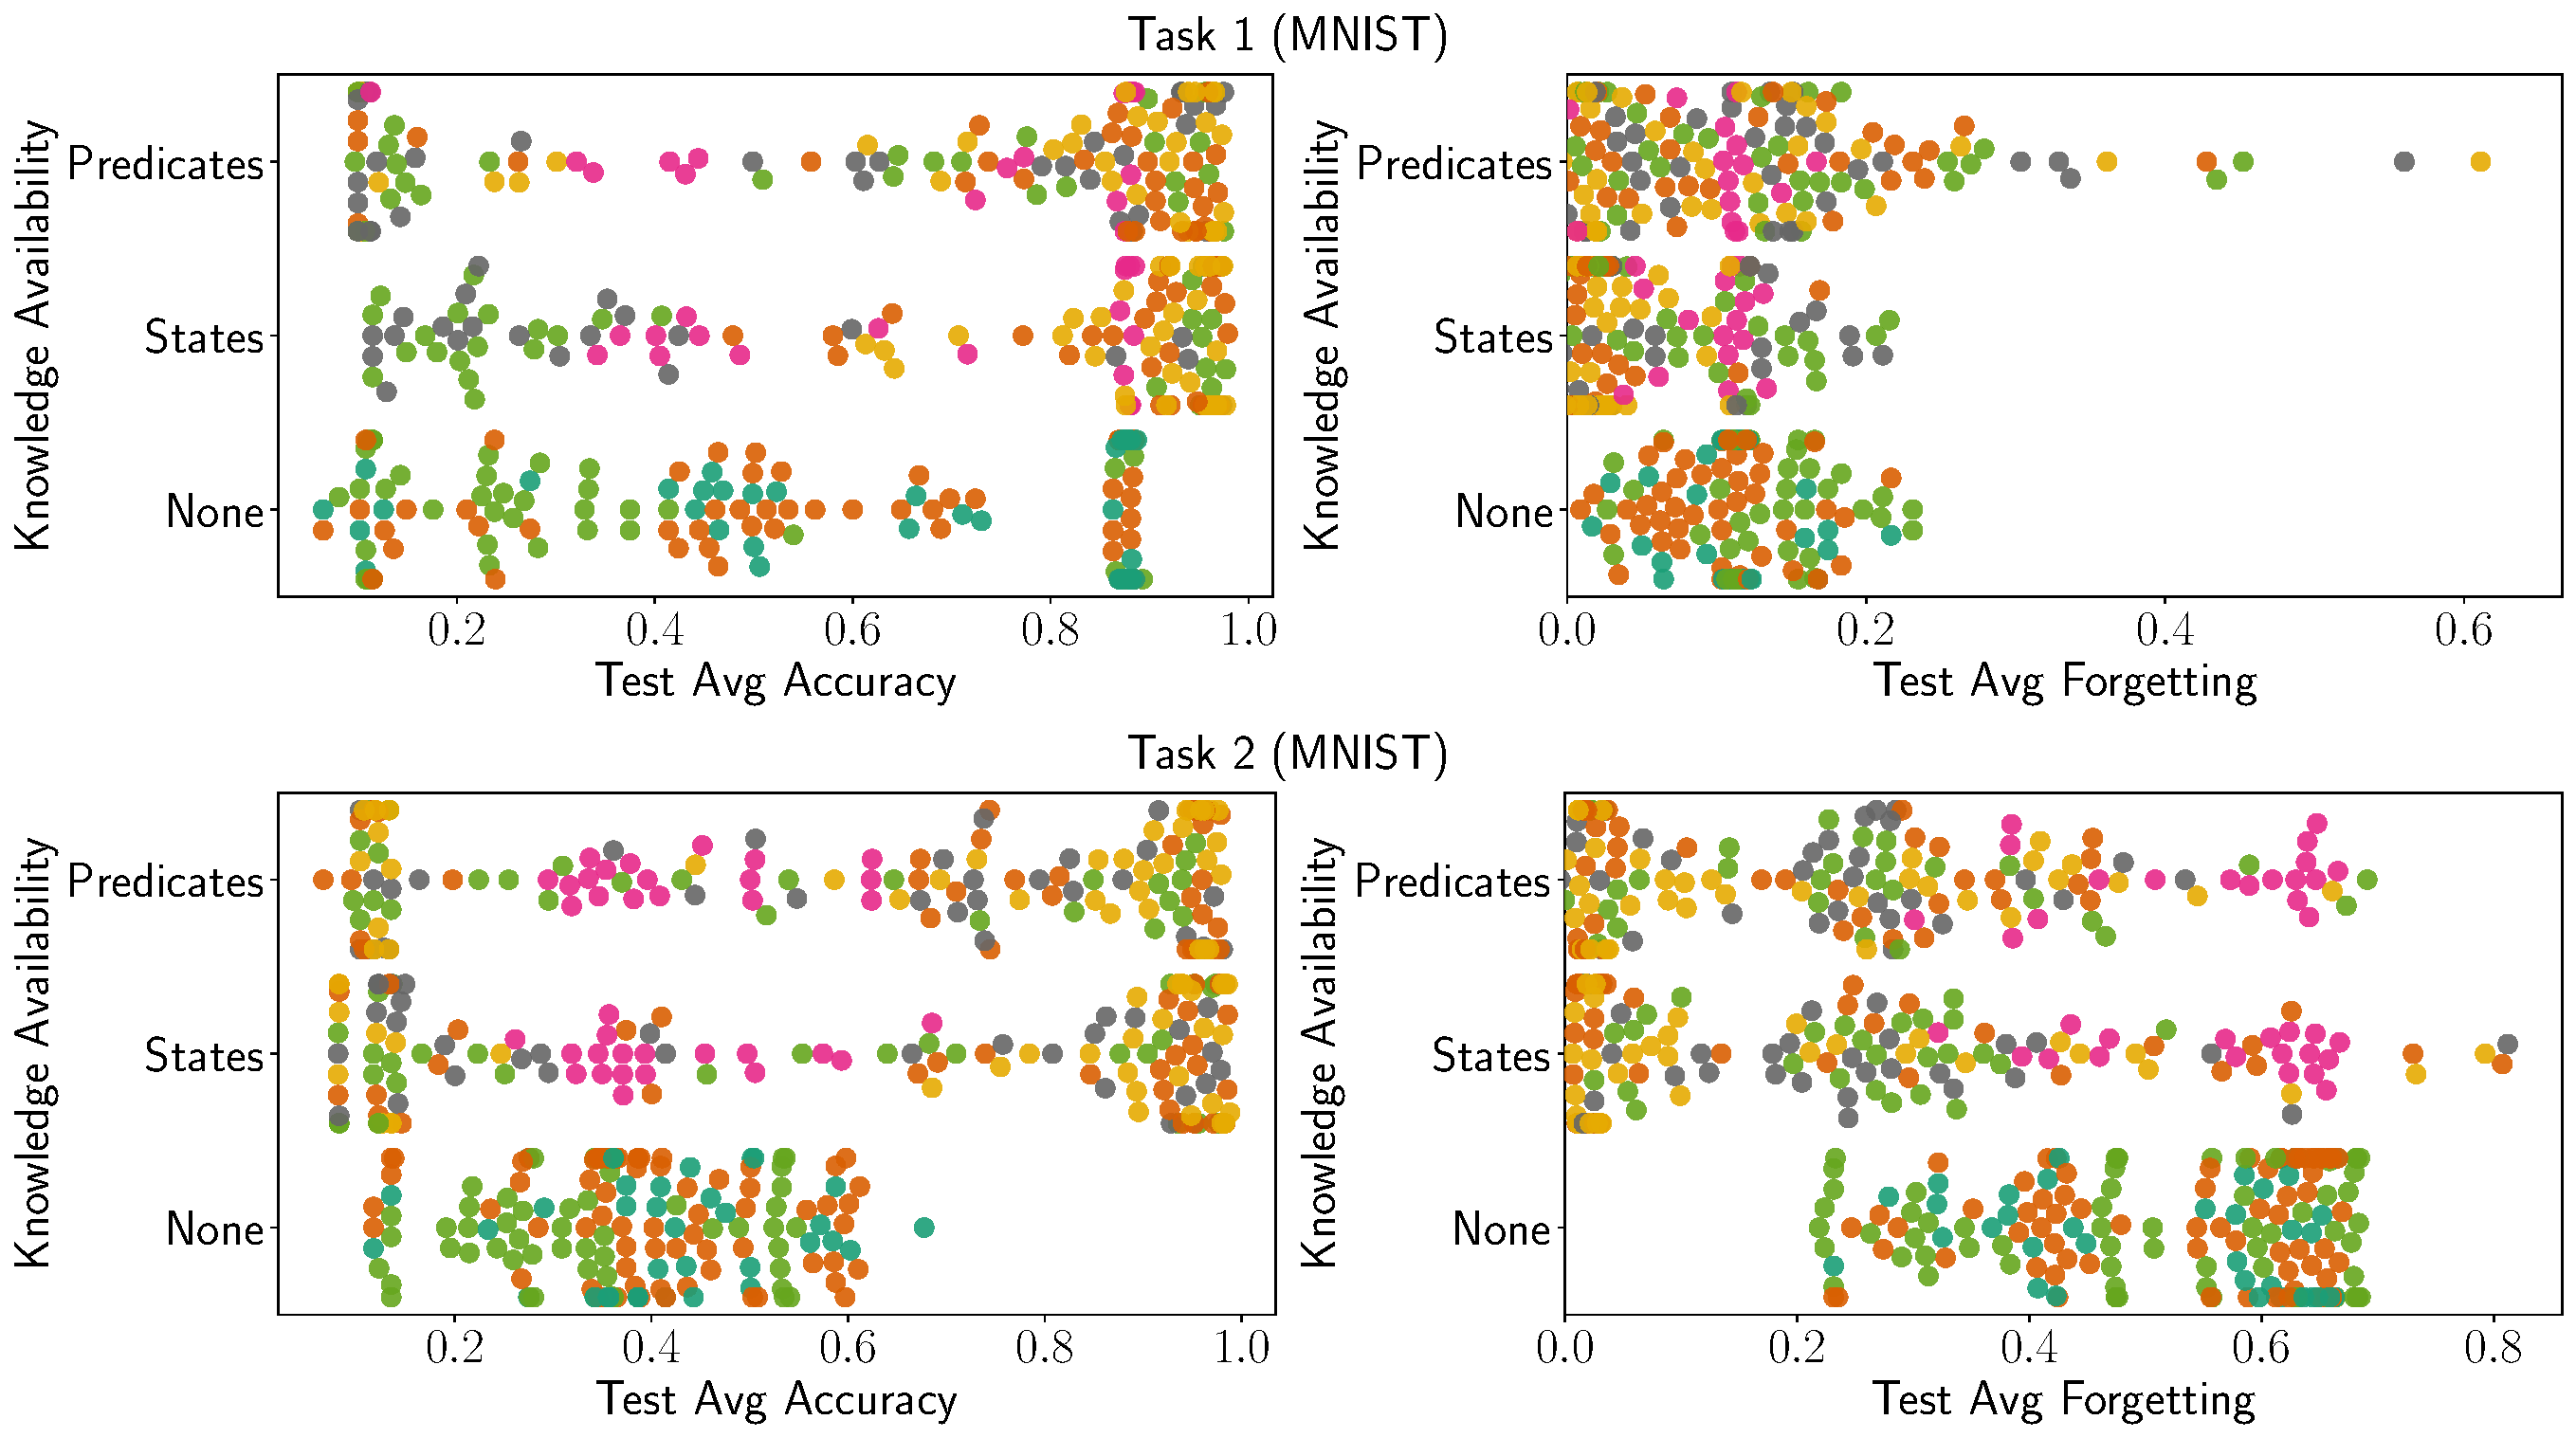
\includegraphics[width=\textwidth]{imgs/ltlzinc/swarm_mnist.pdf}\\
		
\includegraphics[width=\textwidth]{imgs/ltlzinc/swarm_legend.pdf}
	\end{minipage}
	\caption[\textsc{Average Accuracy} and \textsc{Average Forgetting} on \textsc{LTLZinc-Continual-MNIST}]{\textsc{Average Accuracy} and \textsc{Average Forgetting} for Class-continual experiments on \textsc{LTLZinc-Continual-MNIST}, grouped by knowledge available to each strategy.}
	\label{ltlzinc:fig:swarm-mnist}
\end{figure}
%
Figure~\ref{ltlzinc:fig:swarm-mnist} shows \textsc{Average Accuracy} and \textsc{Average Forgetting} of every experiment, grouped by knowledge availability. It can be observed that, although knowledge availability has a potentially positive effect (best methods being able to achieve higher average accuracy and lower average forgetting compared to uninformed strategies), it is not enough on it own, to guarantee good performance (worst methods achieving as bad, for \textsc{Task 1}, or slightly worse, in \textsc{Task 2}, than uninformed baselines), and hyper-parameter tuning plays an equally important role.
When focusing on specific strategies, replay-based methods (and their combinations with other strategies) tend to form tight clusters of high performance (high accuracy, low forgetting) which benefit from available knowledge more than their uninformed counterparts.

\begin{table}
	\centering
	\resizebox{\textwidth}{!}{
		\begin{tabular}{ccccccccccc}
			\toprule
			\multirow{3}{*}{\sc Task} & \multirow{3}{*}{\shortstack[c]{\sc Knowledge\\\sc Availability}} & \multirow{3}{*}{\sc Category} & \multirow{3}{*}{\sc Buffer} & \multirow{3}{*}{\sc Distillation} & \multirow{3}{*}{\sc Architecture} & \multirow{3}{*}{\shortstack[c]{\sc Average\\\sc Accuracy}\raisebox{1.5ex}{\:$\uparrow$}} & \multirow{3}{*}{\shortstack[c]{\sc Average\\\sc Forgetting}\raisebox{1.5ex}{\:$\downarrow$}} & \multirow{3}{*}{\shortstack[c]{\sc Forward\\\sc Transfer}\raisebox{1.5ex}{\:$\uparrow$}} & \multirow{3}{*}{\shortstack[c]{\sc Focused\\\sc Average\\\sc Accuracy}\raisebox{2.5ex}{\:$\uparrow$}} & \multirow{3}{*}{\shortstack[c]{\sc Focused\\\sc Average\\\sc Forgetting}\raisebox{2.5ex}{\:$\downarrow$}} \\
			& & & & & & & & & & \\
			& & & & & & & & & & \\
			\midrule
			
			\multirow{12}{*}{\shortstack[c]{Task 1\\(CIFAR-100)}} & \multirow{4}{*}{Predicates} & Modular & No buffer & No distillation & \multirow{4}{*}{Modular} & $\textbf{0.62} $ {\tiny ($\pm 0.01$)} & $0.06 $ {\tiny ($\pm 0.00$)} & $\textbf{0.50} $ {\tiny ($\pm 0.01$)} & $0.00 $ {\tiny ($\pm 0.00$)} & $0.61 $ {\tiny ($\pm 0.05$)}\\
			&  & Replay + Modular & Reservoir (CCE) & No distillation &  & $0.60 $ {\tiny ($\pm 0.01$)} & $\textbf{0.05} $ {\tiny ($\pm 0.01$)} & $0.49 $ {\tiny ($\pm 0.01$)} & $\textbf{0.27} $ {\tiny ($\pm 0.05$)} & $0.25 $ {\tiny ($\pm 0.06$)}\\
			&  & Distillation + Modular & No buffer & Teacher-distillation &  & $0.61 $ {\tiny ($\pm 0.01$)} & $0.06 $ {\tiny ($\pm 0.01$)} & $0.48 $ {\tiny ($\pm 0.02$)} & $0.00 $ {\tiny ($\pm 0.00$)} & $0.50 $ {\tiny ($\pm 0.08$)}\\
			&  & All & Reservoir (CCE) & Teacher-distillation &  & $0.59 $ {\tiny ($\pm 0.01$)} & $\textbf{0.05} $ {\tiny ($\pm 0.01$)} & $0.47 $ {\tiny ($\pm 0.01$)} & $0.26 $ {\tiny ($\pm 0.06$)} & $\textbf{0.17} $ {\tiny ($\pm 0.07$)}\\
			\cdashline{2-11}
			& \multirow{4}{*}{States} & Modular & No buffer & No distillation & \multirow{4}{*}{Modular} & $\textbf{0.62} $ {\tiny ($\pm 0.01$)} & $0.06 $ {\tiny ($\pm 0.01$)} & $\textbf{0.51} $ {\tiny ($\pm 0.01$)} & $0.00 $ {\tiny ($\pm 0.00$)} & $0.62 $ {\tiny ($\pm 0.07$)}\\
			&  & Replay + Modular & Reservoir (CCE) & No distillation &  & $0.58 $ {\tiny ($\pm 0.02$)} & $\textbf{0.05} $ {\tiny ($\pm 0.01$)} & $0.47 $ {\tiny ($\pm 0.02$)} & $0.18 $ {\tiny ($\pm 0.10$)} & $0.32 $ {\tiny ($\pm 0.07$)}\\
			&  & Distillation + Modular & No buffer & Teacher-distillation &  & $0.62 $ {\tiny ($\pm 0.01$)} & $0.06 $ {\tiny ($\pm 0.01$)} & $0.49 $ {\tiny ($\pm 0.01$)} & $0.00 $ {\tiny ($\pm 0.00$)} & $0.53 $ {\tiny ($\pm 0.04$)}\\
			&  & All & Reservoir (CCE) & Teacher-distillation &  & $0.57 $ {\tiny ($\pm 0.02$)} & $0.06 $ {\tiny ($\pm 0.01$)} & $0.46 $ {\tiny ($\pm 0.02$)} & $\textbf{0.19} $ {\tiny ($\pm 0.10$)} & $\textbf{0.25} $ {\tiny ($\pm 0.09$)}\\
			\cdashline{2-11}
			& \multirow{4}{*}{None} & Naive & No buffer & No distillation & \multirow{4}{*}{Modular} & $\textbf{0.62} $ {\tiny ($\pm 0.01$)} & $\textbf{0.06} $ {\tiny ($\pm 0.01$)} & $\textbf{0.50} $ {\tiny ($\pm 0.01$)} & $0.00 $ {\tiny ($\pm 0.00$)} & $0.62 $ {\tiny ($\pm 0.02$)}\\
			&  & Replay & Reservoir (CCE) & No distillation &  & $\textbf{0.62} $ {\tiny ($\pm 0.01$)} & $\textbf{0.06} $ {\tiny ($\pm 0.01$)} & $\textbf{0.50} $ {\tiny ($\pm 0.01$)} & $0.00 $ {\tiny ($\pm 0.00$)} & $0.61 $ {\tiny ($\pm 0.04$)}\\
			&  & Distillation & No buffer & Self-distillation &  & $\textbf{0.62} $ {\tiny ($\pm 0.01$)} & $\textbf{0.06} $ {\tiny ($\pm 0.01$)} & $0.49 $ {\tiny ($\pm 0.01$)} & $0.00 $ {\tiny ($\pm 0.00$)} & $0.57 $ {\tiny ($\pm 0.05$)}\\
			&  & Replay + Distillation & Reservoir (CCE) & Self-distillation &  & $\textbf{0.62} $ {\tiny ($\pm 0.01$)} & $\textbf{0.06} $ {\tiny ($\pm 0.01$)} & $0.49 $ {\tiny ($\pm 0.01$)} & $0.00 $ {\tiny ($\pm 0.00$)} & $\textbf{0.54} $ {\tiny ($\pm 0.05$)}\\
			\midrule
			\multirow{12}{*}{\shortstack[c]{Task 2\\(CIFAR-100)}} & \multirow{4}{*}{Predicates} & Modular & No buffer & No distillation & \multirow{4}{*}{Modular} & $0.27 $ {\tiny ($\pm 0.09$)} & $0.36 $ {\tiny ($\pm 0.05$)} & $0.17 $ {\tiny ($\pm 0.03$)} & $0.36 $ {\tiny ($\pm 0.25$)} & $0.41 $ {\tiny ($\pm 0.21$)}\\
			&  & Replay + Modular & Reservoir (CCE) & No distillation &  & $0.45 $ {\tiny ($\pm 0.07$)} & $0.15 $ {\tiny ($\pm 0.04$)} & $\textbf{0.38} $ {\tiny ($\pm 0.06$)} & $0.51 $ {\tiny ($\pm 0.13$)} & $0.19 $ {\tiny ($\pm 0.09$)}\\
			&  & Distillation + Modular & No buffer & Teacher-distillation &  & $0.26 $ {\tiny ($\pm 0.08$)} & $0.36 $ {\tiny ($\pm 0.06$)} & $0.16 $ {\tiny ($\pm 0.03$)} & $0.34 $ {\tiny ($\pm 0.24$)} & $0.42 $ {\tiny ($\pm 0.22$)}\\
			&  & All & Reservoir (CCE) & Teacher-distillation &  & $\textbf{0.49} $ {\tiny ($\pm 0.04$)} & $\textbf{0.13} $ {\tiny ($\pm 0.02$)} & $0.35 $ {\tiny ($\pm 0.06$)} & $\textbf{0.58} $ {\tiny ($\pm 0.08$)} & $\textbf{0.15} $ {\tiny ($\pm 0.06$)}\\
			\cdashline{2-11}
			& \multirow{4}{*}{States} & Modular & No buffer & No distillation & \multirow{4}{*}{Modular} & $0.27 $ {\tiny ($\pm 0.09$)} & $0.36 $ {\tiny ($\pm 0.05$)} & $0.17 $ {\tiny ($\pm 0.03$)} & $0.36 $ {\tiny ($\pm 0.25$)} & $0.41 $ {\tiny ($\pm 0.22$)}\\
			&  & Replay + Modular & Reservoir (CCE) & No distillation &  & $\textbf{0.48} $ {\tiny ($\pm 0.05$)} & $\textbf{0.14} $ {\tiny ($\pm 0.02$)} & $\textbf{0.37} $ {\tiny ($\pm 0.05$)} & $\textbf{0.57} $ {\tiny ($\pm 0.10$)} & $\textbf{0.16} $ {\tiny ($\pm 0.07$)}\\
			&  & Distillation + Modular & No buffer & Teacher-distillation &  & $0.25 $ {\tiny ($\pm 0.08$)} & $0.37 $ {\tiny ($\pm 0.05$)} & $0.16 $ {\tiny ($\pm 0.03$)} & $0.32 $ {\tiny ($\pm 0.23$)} & $0.43 $ {\tiny ($\pm 0.21$)}\\
			&  & All & Reservoir (CCE) & Teacher-distillation &  & $\textbf{0.48} $ {\tiny ($\pm 0.03$)} & $\textbf{0.14} $ {\tiny ($\pm 0.02$)} & $0.35 $ {\tiny ($\pm 0.06$)} & $\textbf{0.58} $ {\tiny ($\pm 0.07$)} & $\textbf{0.16} $ {\tiny ($\pm 0.05$)}\\
			\cdashline{2-11}
			& \multirow{4}{*}{None} & Naive & No buffer & No distillation & \multirow{4}{*}{Modular} & $\textbf{0.31} $ {\tiny ($\pm 0.07$)} & $\textbf{0.34} $ {\tiny ($\pm 0.04$)} & $\textbf{0.18} $ {\tiny ($\pm 0.03$)} & $\textbf{0.40} $ {\tiny ($\pm 0.21$)} & $\textbf{0.39} $ {\tiny ($\pm 0.19$)}\\
			&  & Replay & Reservoir (CCE) & No distillation &  & $\textbf{0.31} $ {\tiny ($\pm 0.07$)} & $\textbf{0.34} $ {\tiny ($\pm 0.04$)} & $\textbf{0.18} $ {\tiny ($\pm 0.03$)} & $\textbf{0.40} $ {\tiny ($\pm 0.21$)} & $\textbf{0.39} $ {\tiny ($\pm 0.19$)}\\
			&  & Distillation & No buffer & Self-distillation &  & $0.30 $ {\tiny ($\pm 0.06$)} & $0.37 $ {\tiny ($\pm 0.05$)} & $0.17 $ {\tiny ($\pm 0.02$)} & $0.38 $ {\tiny ($\pm 0.24$)} & $0.43 $ {\tiny ($\pm 0.22$)}\\
			&  & Replay + Distillation & Reservoir (CCE) & Self-distillation &  & $0.30 $ {\tiny ($\pm 0.07$)} & $0.38 $ {\tiny ($\pm 0.05$)} & $0.17 $ {\tiny ($\pm 0.03$)} & $0.37 $ {\tiny ($\pm 0.25$)} & $0.43 $ {\tiny ($\pm 0.23$)}\\
			\bottomrule
		\end{tabular}
	}
	\caption[Results on \textsc{LTLZinc-Continual-CIFAR}]{Best \textsc{Average Accuracy}, \textsc{Average Forgetting} and \textsc{Forward Transfer} for Class-continual experiments on \textsc{LTLZinc-Continual-CIFAR} with trainable backbone, grouped by knowledge available to each strategy. Best models selected by \textsc{Average Accuracy} on validation set. Results are $mean \pm std$ over 9 runs (3 random seeds, times 3 different curricula).}
	\label{ltlzinc:tab:incremental-results-cifar}
\end{table}

\begin{figure}
	\centering
	\begin{minipage}{\linewidth}
		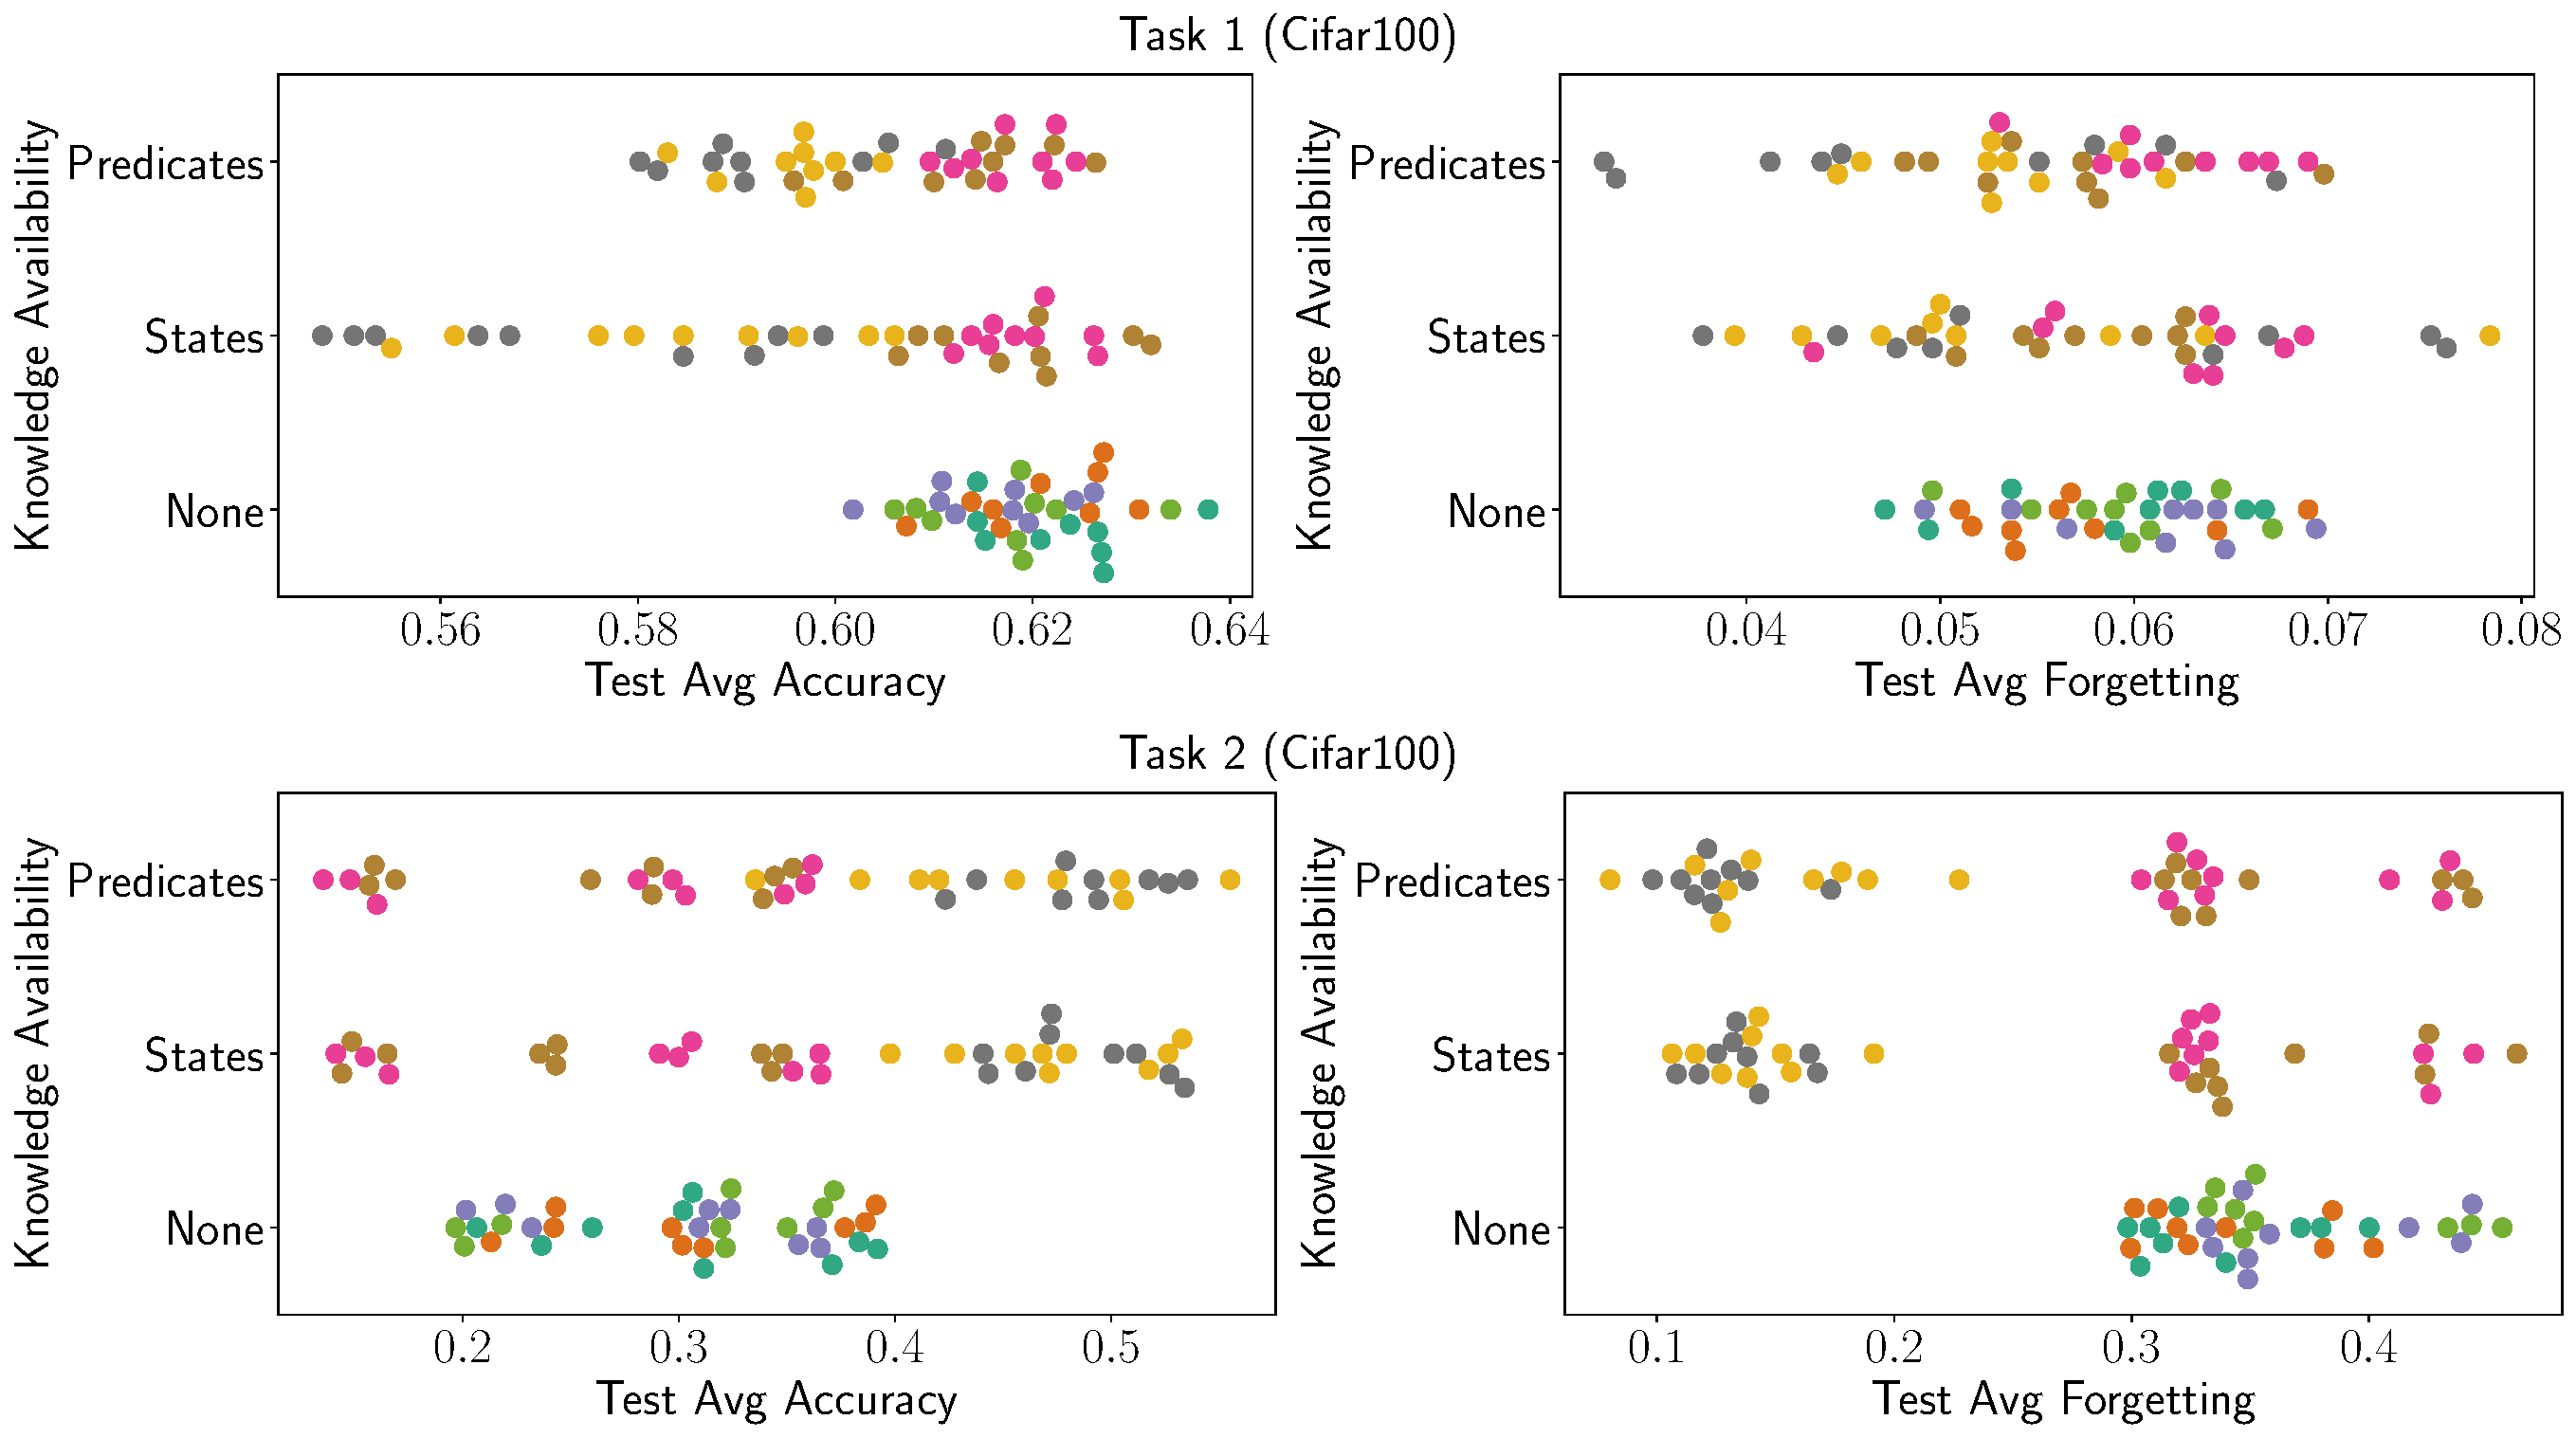
\includegraphics[width=\textwidth]{imgs/ltlzinc/swarm_cifar.pdf}\\
		
\includegraphics[width=\textwidth]{imgs/ltlzinc/swarm_legend.pdf}
	\end{minipage}
	\caption[\textsc{Average Accuracy} and \textsc{Average Forgetting} on \textsc{LTLZinc-Continual-CIFAR}]{\textsc{Average Accuracy} and \textsc{Average Forgetting} for Class-continual experiments on \textsc{LTLZinc-Continual-CIFAR} with trainable backbone, grouped by knowledge available to each strategy.}
	\label{ltlzinc:fig:swarm-cifar}
\end{figure}

\paragraph{\textsc{LTLZinc-Continual-CIFAR}.} Table~\ref{ltlzinc:tab:incremental-results-cifar} and Figure~\ref{ltlzinc:fig:swarm-cifar} correspond to \textsc{LTLZinc-Continual-CIFAR} experiments with a trainable backbone.
Also in this case, characterized by more complex perceptual features and 100 classes, we observe a performance significantly above random guessing ($0.01$ accuracy) for every method, but differences at the level of global metrics (\textsc{Average Accuracy}, \textsc{Average Forgetting}, \textsc{Forward Transfer}) are virtually non-existent for \textsc{Task 1}, while for \textsc{Task 2}, uninformed strategies position themselves between good and bad knowledge-driven strategies, making it impossible to draw strong conclusions on the effect of knowledge availability. This phenomenon can be explained only in part by the more challenging setting, and it is more likely due to weights pre-trained on ImageNet (which presents perceptual features easily adaptable to CIFAR-100). However, a different scenario is captured by focused metrics. For \textsc{Task 1} it can be observed how exploiting background knowledge is the only way to avoid catastrophic forgetting on rare labels (even though there are some bad combinations which still fail to classify them by the end of training).
Like in the case of \textsc{LTLZinc-Continual-MNIST}, metrics on re-occurring labels (\textsc{Task 2}) do not provide additional information, compared to global metrics.
We can observe from Figure~\ref{ltlzinc:fig:swarm-cifar} that different strategies interact with available knowledge in completely different ways for the two tasks: while replay-based methods are penalized by knowledge in \textsc{Task 1}, they seem to perform overall better in \textsc{Task 2} if they are allowed to exploit knowledge.
Table~\ref{ltlzinc:tab:incremental-results-cifar-frozen} and Figure~\ref{ltlzinc:fig:swarm-cifar-frozen} refer to \textsc{LTLZinc-Continual-CIFAR} experiments with frozen backbone. Although with overall lower scores, the trends identified in experiments with a trainable backbone are confirmed, hinting for an effect of continual adaptation over time that is mostly localized at the final layers.
\begin{table}
	\centering
	\resizebox{\textwidth}{!}{
		\begin{tabular}{ccccccccccc}
			\toprule
			\multirow{3}{*}{\sc Task} & \multirow{3}{*}{\shortstack[c]{\sc Knowledge\\\sc Availability}} & \multirow{3}{*}{\sc Category} & \multirow{3}{*}{\sc Buffer} & \multirow{3}{*}{\sc Distillation} & \multirow{3}{*}{\sc Architecture} & \multirow{3}{*}{\shortstack[c]{\sc Average\\\sc Accuracy}\raisebox{1.5ex}{\:$\uparrow$}} & \multirow{3}{*}{\shortstack[c]{\sc Average\\\sc Forgetting}\raisebox{1.5ex}{\:$\downarrow$}} & \multirow{3}{*}{\shortstack[c]{\sc Forward\\\sc Transfer}\raisebox{1.5ex}{\:$\uparrow$}} & \multirow{3}{*}{\shortstack[c]{\sc Focused\\\sc Average\\\sc Accuracy}\raisebox{2.5ex}{\:$\uparrow$}} & \multirow{3}{*}{\shortstack[c]{\sc Focused\\\sc Average\\\sc Forgetting}\raisebox{2.5ex}{\:$\downarrow$}} \\
			& & & & & & & & & & \\
			& & & & & & & & & & \\
			\midrule
			\multirow{12}{*}{\shortstack[c]{Task 1\\(CIFAR-100)\\{[frozen]}}} & \multirow{4}{*}{Predicates} & Modular & No buffer & No distillation & \multirow{4}{*}{Modular} & $\textbf{0.50} $ {\tiny ($\pm 0.01$)} & $0.07 $ {\tiny ($\pm 0.01$)} & $\textbf{0.44} $ {\tiny ($\pm 0.01$)} & $0.00 $ {\tiny ($\pm 0.00$)} & $0.52 $ {\tiny ($\pm 0.03$)}\\
			&  & Replay + Modular & Reservoir (CCE) & No distillation &  & $0.48 $ {\tiny ($\pm 0.01$)} & $\textbf{0.06} $ {\tiny ($\pm 0.01$)} & $0.42 $ {\tiny ($\pm 0.01$)} & $\textbf{0.24} $ {\tiny ($\pm 0.05$)} & $\textbf{0.20} $ {\tiny ($\pm 0.05$)}\\
			&  & Distillation + Modular & No buffer & Teacher-distillation &  & $\textbf{0.50} $ {\tiny ($\pm 0.01$)} & $0.07 $ {\tiny ($\pm 0.00$)} & $\textbf{0.44} $ {\tiny ($\pm 0.01$)} & $0.00 $ {\tiny ($\pm 0.00$)} & $0.46 $ {\tiny ($\pm 0.03$)}\\
			&  & All & Reservoir (CCE) & Teacher-distillation &  & $0.48 $ {\tiny ($\pm 0.01$)} & $\textbf{0.06} $ {\tiny ($\pm 0.01$)} & $0.42 $ {\tiny ($\pm 0.01$)} & $\textbf{0.24} $ {\tiny ($\pm 0.05$)} & $\textbf{0.20} $ {\tiny ($\pm 0.04$)}\\
			\cdashline{2-11}
			& \multirow{4}{*}{States} & Modular & No buffer & No distillation & \multirow{4}{*}{Modular} & $\textbf{0.50} $ {\tiny ($\pm 0.01$)} & $0.06 $ {\tiny ($\pm 0.00$)} & $\textbf{0.44} $ {\tiny ($\pm 0.01$)} & $0.00 $ {\tiny ($\pm 0.00$)} & $0.52 $ {\tiny ($\pm 0.03$)}\\
			&  & Replay + Modular & Reservoir (CCE) & No distillation &  & $0.48 $ {\tiny ($\pm 0.01$)} & $0.06 $ {\tiny ($\pm 0.01$)} & $0.41 $ {\tiny ($\pm 0.01$)} & $\textbf{0.18} $ {\tiny ($\pm 0.08$)} & $0.24 $ {\tiny ($\pm 0.09$)}\\
			&  & Distillation + Modular & No buffer & Teacher-distillation &  & $\textbf{0.50} $ {\tiny ($\pm 0.01$)} & $0.07 $ {\tiny ($\pm 0.00$)} & $\textbf{0.44} $ {\tiny ($\pm 0.01$)} & $0.00 $ {\tiny ($\pm 0.00$)} & $0.47 $ {\tiny ($\pm 0.03$)}\\
			&  & All & Reservoir (CCE) & Teacher-distillation &  & $0.48 $ {\tiny ($\pm 0.01$)} & $\textbf{0.05} $ {\tiny ($\pm 0.01$)} & $0.41 $ {\tiny ($\pm 0.01$)} & $0.17 $ {\tiny ($\pm 0.08$)} & $\textbf{0.22} $ {\tiny ($\pm 0.07$)}\\
			\cdashline{2-11}
			& \multirow{4}{*}{None} & Naive & No buffer & No distillation & \multirow{4}{*}{Modular} & $\textbf{0.52} $ {\tiny ($\pm 0.01$)} & $0.06 $ {\tiny ($\pm 0.01$)} & $\textbf{0.44} $ {\tiny ($\pm 0.01$)} & $0.00 $ {\tiny ($\pm 0.00$)} & $0.49 $ {\tiny ($\pm 0.04$)}\\
			&  & Replay & Reservoir (CCE) & No distillation &  & $\textbf{0.52} $ {\tiny ($\pm 0.01$)} & $0.06 $ {\tiny ($\pm 0.00$)} & $\textbf{0.44} $ {\tiny ($\pm 0.01$)} & $0.00 $ {\tiny ($\pm 0.00$)} & $0.49 $ {\tiny ($\pm 0.03$)}\\
			&  & Distillation & No buffer & Self-distillation &  & $\textbf{0.52} $ {\tiny ($\pm 0.00$)} & $\textbf{0.05} $ {\tiny ($\pm 0.00$)} & $0.43 $ {\tiny ($\pm 0.01$)} & $0.00 $ {\tiny ($\pm 0.00$)} & $0.45 $ {\tiny ($\pm 0.05$)}\\
			&  & Replay + Distillation & Reservoir (CCE) & Self-distillation &  & $\textbf{0.52} $ {\tiny ($\pm 0.00$)} & $\textbf{0.05} $ {\tiny ($\pm 0.00$)} & $0.43 $ {\tiny ($\pm 0.01$)} & $0.00 $ {\tiny ($\pm 0.00$)} & $\textbf{0.44} $ {\tiny ($\pm 0.05$)}\\
			\midrule
			\multirow{12}{*}{\shortstack[c]{Task 2\\(CIFAR-100)\\{[frozen]}}} & \multirow{4}{*}{Predicates} & Modular & No buffer & No distillation & \multirow{4}{*}{Modular} & $0.29 $ {\tiny ($\pm 0.03$)} & $0.34 $ {\tiny ($\pm 0.03$)} & $0.20 $ {\tiny ($\pm 0.01$)} & $0.34 $ {\tiny ($\pm 0.19$)} & $0.37 $ {\tiny ($\pm 0.18$)}\\
			&  & Replay + Modular & Reservoir (CCE) & No distillation &  & $\textbf{0.43} $ {\tiny ($\pm 0.02$)} & $\textbf{0.13} $ {\tiny ($\pm 0.01$)} & $\textbf{0.37} $ {\tiny ($\pm 0.02$)} & $\textbf{0.49} $ {\tiny ($\pm 0.06$)} & $\textbf{0.15} $ {\tiny ($\pm 0.06$)}\\
			&  & Distillation + Modular & No buffer & Teacher-distillation &  & $0.28 $ {\tiny ($\pm 0.03$)} & $0.34 $ {\tiny ($\pm 0.02$)} & $0.17 $ {\tiny ($\pm 0.02$)} & $0.33 $ {\tiny ($\pm 0.19$)} & $0.37 $ {\tiny ($\pm 0.18$)}\\
			&  & All & Reservoir (CCE) & Teacher-distillation &  & $\textbf{0.43} $ {\tiny ($\pm 0.02$)} & $0.14 $ {\tiny ($\pm 0.01$)} & $0.35 $ {\tiny ($\pm 0.03$)} & $\textbf{0.49} $ {\tiny ($\pm 0.06$)} & $0.16 $ {\tiny ($\pm 0.06$)}\\
			\cdashline{2-11}
			& \multirow{4}{*}{States} & Modular & No buffer & No distillation & \multirow{4}{*}{Modular} & $0.31 $ {\tiny ($\pm 0.03$)} & $0.32 $ {\tiny ($\pm 0.02$)} & $0.20 $ {\tiny ($\pm 0.01$)} & $0.36 $ {\tiny ($\pm 0.18$)} & $0.35 $ {\tiny ($\pm 0.17$)}\\
			&  & Replay + Modular & Reservoir (CCE) & No distillation &  & $0.41 $ {\tiny ($\pm 0.01$)} & $0.15 $ {\tiny ($\pm 0.01$)} & $\textbf{0.34} $ {\tiny ($\pm 0.02$)} & $0.48 $ {\tiny ($\pm 0.04$)} & $0.16 $ {\tiny ($\pm 0.04$)}\\
			&  & Distillation + Modular & No buffer & Teacher-distillation &  & $0.29 $ {\tiny ($\pm 0.03$)} & $0.34 $ {\tiny ($\pm 0.02$)} & $0.18 $ {\tiny ($\pm 0.02$)} & $0.34 $ {\tiny ($\pm 0.18$)} & $0.37 $ {\tiny ($\pm 0.17$)}\\
			&  & All & Reservoir (CCE) & Teacher-distillation &  & $\textbf{0.43} $ {\tiny ($\pm 0.01$)} & $\textbf{0.14} $ {\tiny ($\pm 0.01$)} & $0.33 $ {\tiny ($\pm 0.03$)} & $\textbf{0.50} $ {\tiny ($\pm 0.05$)} & $\textbf{0.15} $ {\tiny ($\pm 0.05$)}\\
			\cdashline{2-11}
			& \multirow{4}{*}{None} & Naive & No buffer & No distillation & \multirow{4}{*}{Modular} & $\textbf{0.30} $ {\tiny ($\pm 0.02$)} & $\textbf{0.34} $ {\tiny ($\pm 0.02$)} & $\textbf{0.19} $ {\tiny ($\pm 0.01$)} & $\textbf{0.35} $ {\tiny ($\pm 0.18$)} & $\textbf{0.37} $ {\tiny ($\pm 0.17$)}\\
			&  & Replay & Reservoir (CCE) & No distillation &  & $\textbf{0.30} $ {\tiny ($\pm 0.02$)} & $\textbf{0.34} $ {\tiny ($\pm 0.01$)} & $\textbf{0.19} $ {\tiny ($\pm 0.01$)} & $\textbf{0.35} $ {\tiny ($\pm 0.18$)} & $\textbf{0.37} $ {\tiny ($\pm 0.17$)}\\
			&  & Distillation & No buffer & Self-distillation &  & $0.28 $ {\tiny ($\pm 0.03$)} & $0.35 $ {\tiny ($\pm 0.02$)} & $0.17 $ {\tiny ($\pm 0.01$)} & $0.34 $ {\tiny ($\pm 0.20$)} & $0.38 $ {\tiny ($\pm 0.18$)}\\
			&  & Replay + Distillation & Reservoir (CCE) & Self-distillation &  & $0.29 $ {\tiny ($\pm 0.03$)} & $0.35 $ {\tiny ($\pm 0.02$)} & $0.17 $ {\tiny ($\pm 0.01$)} & $0.34 $ {\tiny ($\pm 0.19$)} & $0.38 $ {\tiny ($\pm 0.18$)}\\
			
			\bottomrule
		\end{tabular}
	}
	\caption[Results on \textsc{LTLZinc-Continual-CIFAR} (frozen backbone)]{Best \textsc{Average Accuracy}, \textsc{Average Forgetting} and \textsc{Forward Transfer} for Class-continual experiments on \textsc{LTLZinc-Continual-CIFAR} with frozen backbone, grouped by knowledge available to each strategy. Best models selected by \textsc{Average Accuracy} on validation set. Results are $mean \pm std$ over 9 runs (3 random seeds, times 3 different curricula).}
	\label{ltlzinc:tab:incremental-results-cifar-frozen}
\end{table}

\begin{figure}
	\centering
	\begin{minipage}{\linewidth}
		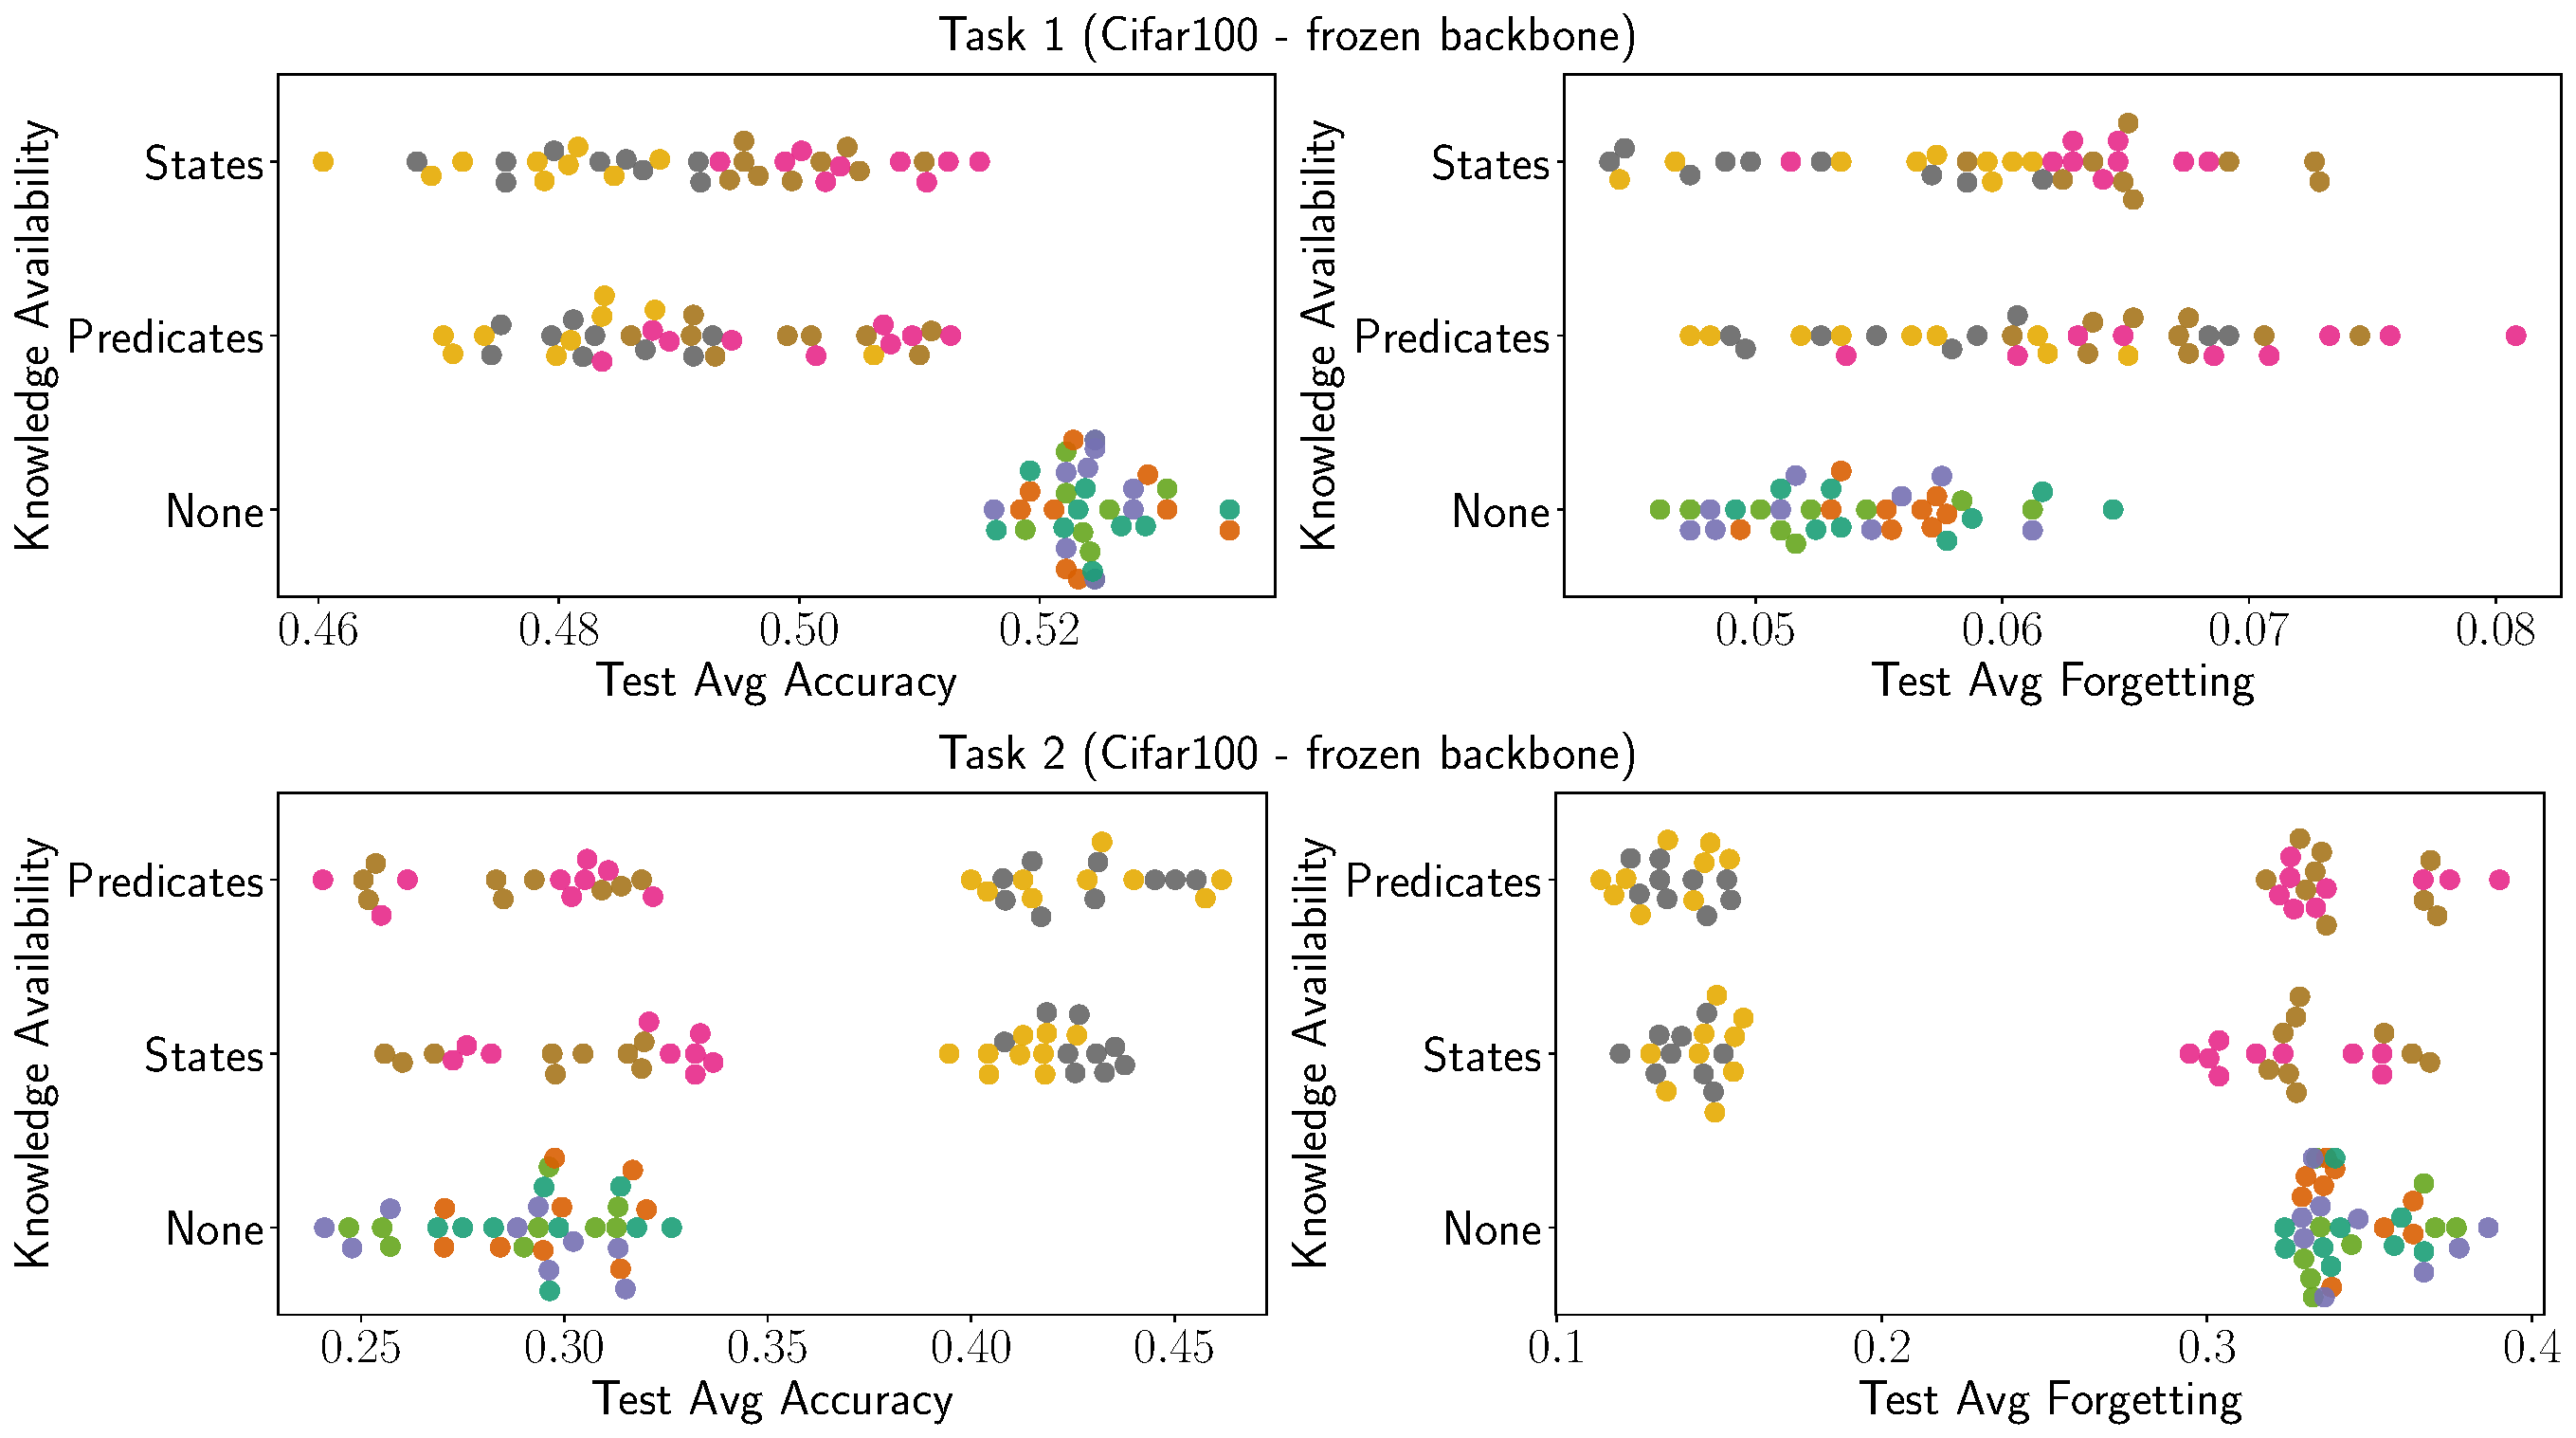
\includegraphics[width=\textwidth]{imgs/ltlzinc/swarm_cifar_frozen.pdf}\\
		
\includegraphics[width=\textwidth]{imgs/ltlzinc/swarm_legend.pdf}
	\end{minipage}
	\caption[\textsc{Average Accuracy} and \textsc{Average Forgetting} on \textsc{LTLZinc-Continual-CIFAR} (frozen backbone)]{\textsc{Average Accuracy} and \textsc{Average Forgetting} for Class-continual experiments on \textsc{LTLZinc-Continual-CIFAR} with frozen backbone, grouped by knowledge available to each strategy.}
	\label{ltlzinc:fig:swarm-cifar-frozen}
\end{figure}
